\subsection{Erosion}
Figur~\ref{fig:erosion1} og \ref{fig:erosion2} viser erosion.

Erosion bruger et \textit{structuring element} også kendt som en \textit{template}. Når dette element placeres i en større figur, som vist i Figur~\ref{fig:erosion1} vil den kun beholde de elementer som midten af \textit{strel} elementet kunne nå. Alt andet fjernes.

\textbf{Bruges ofte til at fjerne mindre ting}. Eksempel kan ses på Figur~\ref{fig:erosion-in-use}.

\begin{figure}[H]
	\centering
	
\includegraphics[width=0.8\linewidth]{figs/spm09/erosion-in-use}
	\caption{Erosion i brug.}
	\label{fig:erosion-in-use}
\end{figure}

\begin{figure}[H]
	\centering
	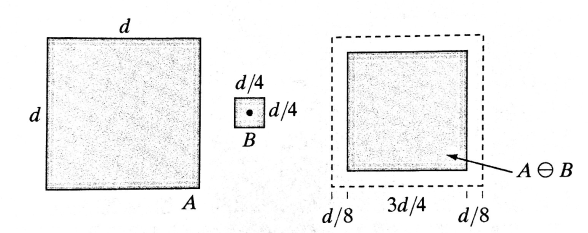
\includegraphics[width=0.7\linewidth]{figs/spm09/erosion1}
	\caption{Eksempel på erosion med 4x4 strel.}
	\label{fig:erosion1}
\end{figure}

\begin{figure}[H]
	\centering
	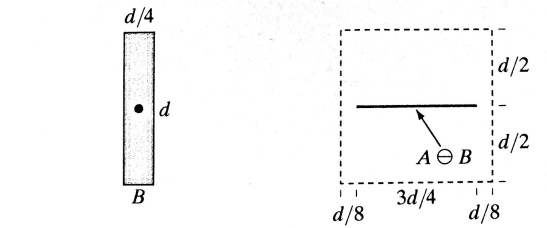
\includegraphics[width=0.7\linewidth]{figs/spm09/erosion2}
	\caption{Eksempel på erosion med aflangt strel.}
	\label{fig:erosion2}
\end{figure}

Matematisk vil udtrykker være som vist i Figur~\ref{fig:erosioneq1}. 

\begin{figure}[H]
	\centering
	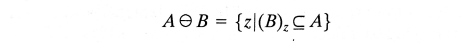
\includegraphics[width=0.7\linewidth]{figs/spm09/erosioneq1}
	\caption{Ligning for erosion.}
	\label{fig:erosioneq1}
\end{figure}

Figur~\ref{fig:erosioneq2} er også er fint udtryk for erosion. Da forskellen bare er at B ikke må have noget tilfælles med baggrunden, i stedet for at den skal have alle punkter tilfælles med A.

\begin{figure}[H]
	\centering
	
\includegraphics[width=0.66\linewidth]{figs/spm09/erosioneq2}
	\caption{Ligning for erosion.}
	\label{fig:erosioneq2}
\end{figure}
